\iffalse
\let\negmedspace\undefined
\let\negthickspace\undefined
\documentclass[journal,12pt,twocolumn]{IEEEtran}
\usepackage{cite}
\usepackage{amsmath,amssymb,amsfonts,amsthm}
\usepackage{algorithmic}
\usepackage{graphicx}
\usepackage{textcomp}
\usepackage{xcolor}
\usepackage{txfonts}
\usepackage{listings}
\usepackage{enumitem}
\usepackage{mathtools}
\usepackage{gensymb}
\usepackage{comment}
\usepackage[breaklinks=true]{hyperref}
\usepackage{tkz-euclide} 
\usepackage{listings}
\usepackage{gvv}                                        
\def\inputGnumericTable{}                                 
\usepackage[latin1]{inputenc}                                
\usepackage{color}                                            
\usepackage{array}                                            
\usepackage{longtable}                                       
\usepackage{calc}                                             
\usepackage{multirow}                                         
\usepackage{hhline}                                           
\usepackage{ifthen}                                           
\usepackage{lscape}
\usepackage{circuitikz}
\newtheorem{theorem}{Theorem}[section]
\newtheorem{problem}{Problem}
\newtheorem{proposition}{Proposition}[section]
\newtheorem{lemma}{Lemma}[section]
\newtheorem{corollary}[theorem]{Corollary}
\newtheorem{example}{Example}[section]
\newtheorem{definition}[problem]{Definition}
\newcommand{\BEQA}{\begin{eqnarray}}
\newcommand{\EEQA}{\end{eqnarray}}
\newcommand{\define}{\stackrel{\triangle}{=}}
\theoremstyle{remark}
\newtheorem{rem}{Remark}
\begin{document}
\parindent 0px

\bibliographystyle{IEEEtran}
\vspace{3cm}

\title{Assignment\\[1ex]GATE-EC-39}
\author{EE23BTECH11034 - Prabhat Kukunuri$^{}$% <-this % stops a space
}
\maketitle
\newpage
\bigskip

\renewcommand{\thefigure}{\theenumi}
\renewcommand{\thetable}{\theenumi}
\section{Question}
Consider the circuit shown in the figure with input V(t) in volts.The sinusoidal steady state current I(t) flowing through the circuit is shown graphically(where t is in seconds). The circuit element Z can be\rule{1.5cm}{0.15mm}.
\begin{enumerate}
    \item a capacitor of 1 F
    \item an inductor of 1 H
    \item a capacitor of $\sqrt{3}$ H
    \item an inductor of $\sqrt{3}$ H
\end{enumerate}
\begin{circuitikz}
    \draw (0,0) node[ground]{};
    \draw (0,0) to [sV, l=$v(t)$] (0,3);
    \draw (0,3) to [resistor, l=$R$,i>^=$I(t)$] (3,3);
    \draw (3,3)to[european resistor,l=$Z$] (3,0);
    \draw (0,0)to (3,0);
  \end{circuitikz}
\begin{figure}[ht]
    \centering
    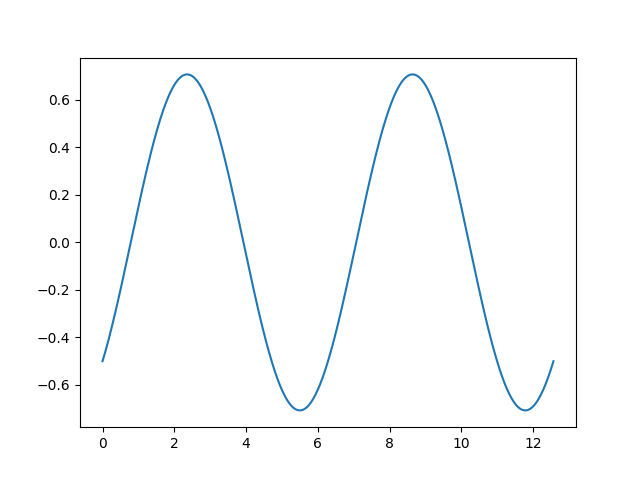
\includegraphics[width=\columnwidth]{2022/EC/39/figs/sin.png}
    \label{fig:GATE.2022.EC.39.1}
\end{figure}


\solution\\
\fi
\begin{table}[h]
    \centering
    \begin{tabular}{|p{2cm}|p{2.80cm}|p{2.70cm}|}
    \hline
    Symbol&Value&Description\\ \hline
    $$V\brak{t}$$&$$\sin{t}$$&Time varying voltage source\\\hline
    $$I\brak{t}$$&$$\sin{t-\frac{\pi}{4}}$$&Current flowing in the circuit\\\hline
    $$R$$&$$1\ohm$$&Resistor in series to Z\\\hline
    $$Z$$&$$Z$$&Circuit element\\\hline
    \end{tabular}
    \caption{Variable description}
    \label{tab:GATE.2022.EC.39.1}
\end{table}\\
The current through the circuit can be expressed as
\begin{align}
    I(t)=\sin\brak{t-\frac{\pi}{4}}
\end{align}
Since, the voltage seems to be leading the current the circuit element z is an inductor with inductance L.\\
Applying KVL in the circuit,
\begin{align}
    R.I\brak{t}+L\frac{dI\brak{t}}{dt}=sin\brak{t}
\end{align}
Applying Fourier transform to the differential equation,
\begin{align}
    &R.I\brak{s}+sL.I\brak{s}-\frac{1}{s^2+1}=0\\
    &I\brak{s}\brak{R+sL}=\frac{1}{s^2+1}\\
    &\sin\brak{at+b}\system{L}\frac{a\cos\brak{b}+s\sin\brak{b}}{a^{2}+s^{2}}\\
    &\sin\brak{t-\frac{\pi}{4}}\system{L}\frac{1-s}{2\brak{s^2+1}}\\
    &\frac{1-s}{2\brak{s^2+1}}\brak{R+sL}=\frac{1}{s^2+1}
\end{align}
Upon plugging in R=1$\ohm$,
\begin{align}
   L=\frac{1}{s}
\end{align}
Applying inverse Laplace,
\begin{align}
    L=1H
\end{align}
%\end{document}
